% Fig. 1 of the revised manuscript: how a model reaches the GPU.
% Build: sh paper/figures/build_architecture.sh  (writes fig_architecture.pdf)
\documentclass[tikz,border=4pt]{standalone}
\usepackage[T1]{fontenc}
\usepackage{lmodern}
\usetikzlibrary{positioning,arrows.meta,fit,backgrounds,calc}
\begin{document}
\sffamily\small
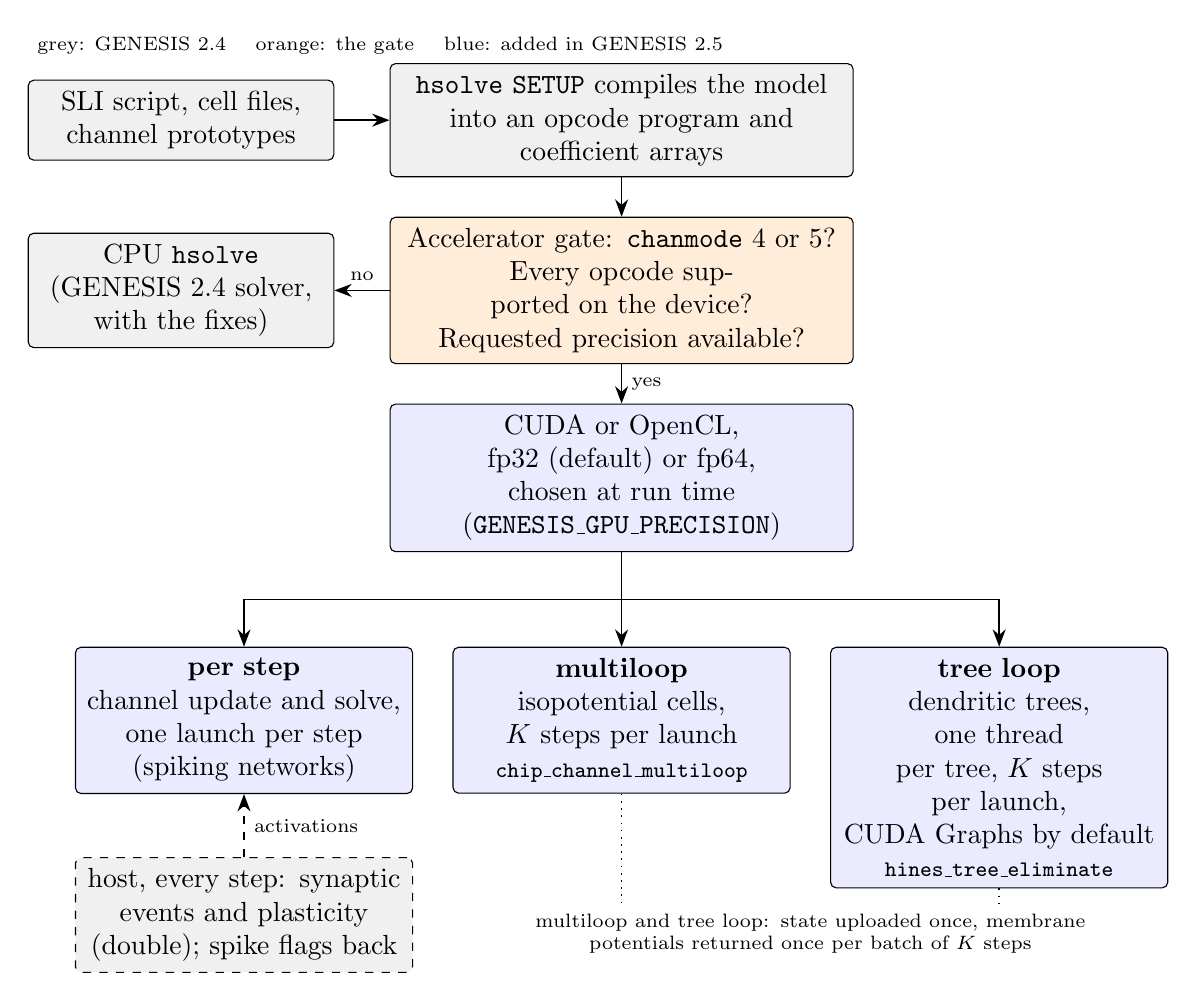
\begin{tikzpicture}[
    box/.style={draw, rounded corners=2pt, align=center, inner sep=4pt, minimum height=9mm},
    old/.style={box, fill=black!6},
    new/.style={box, fill=blue!8},
    gate/.style={box, fill=orange!15},
    host/.style={box, fill=black!6, dashed},
    arr/.style={-{Stealth[length=2.2mm]}, semithick},
    lab/.style={font=\scriptsize, align=center},
    node distance=5mm and 7mm]

% --- unchanged GENESIS
\node[old, text width=36mm] (model) {SLI script, cell files,\\channel prototypes};
\node[old, text width=56mm, right=of model] (setup)
    {\texttt{hsolve SETUP} compiles the model\\into an opcode program and\\coefficient arrays};
\draw[arr] (model) -- (setup);

% --- gate
\node[gate, text width=56mm, below=of setup] (gate)
    {Accelerator gate: \texttt{chanmode} 4 or 5?\\Every opcode supported on the device?\\Requested precision available?};
\draw[arr] (setup) -- (gate);
\node[old, text width=36mm, left=of gate] (cpu)
    {CPU \texttt{hsolve}\\(GENESIS 2.4 solver,\\with the fixes)};
\draw[arr] (gate) -- node[lab, above]{no} (cpu);

% --- backends
\node[new, text width=56mm, below=of gate] (backend)
    {CUDA or OpenCL, fp32 (default) or fp64,\\chosen at run time\\(\texttt{GENESIS\_GPU\_PRECISION})};
\draw[arr] (gate) -- node[lab, right]{yes} (backend);

% --- three dispatch paths, tops aligned
\coordinate (row) at ([yshift=-12mm]backend.south);
\node[new, text width=40mm, anchor=north] (multi) at (row)
    {\textbf{multiloop}\\isopotential cells,\\$K$ steps per launch\\{\footnotesize\texttt{chip\_channel\_multiloop}}};
\node[new, text width=40mm, anchor=north east] (step) at ([xshift=-5mm]multi.north west)
    {\textbf{per step}\\channel update and solve,\\one launch per step\\(spiking networks)};
\node[new, text width=40mm, anchor=north west] (tree) at ([xshift=5mm]multi.north east)
    {\textbf{tree loop}\\dendritic trees, one thread\\per tree, $K$ steps per launch,\\CUDA Graphs by default\\{\footnotesize\texttt{hines\_tree\_eliminate}}};
\draw[arr] (backend.south) -- ++(0,-6mm) -| (step.north);
\draw[arr] (backend.south) -- (multi.north);
\draw[arr] (backend.south) -- ++(0,-6mm) -| (tree.north);

% --- host side, every step for networks
\node[host, text width=40mm, below=8mm of step] (events)
    {host, every step: synaptic\\events and plasticity\\(double); spike flags back};
\draw[arr, dashed] (events.north) -- node[lab, right]{activations} (step.south);

% --- transfers
\node[lab, text width=85mm, anchor=north] (xfer) at ([yshift=-8mm]$(multi.south)!0.5!(tree.south)$)
    {multiloop and tree loop: state uploaded once, membrane\\potentials returned once per batch of $K$ steps};
\draw[semithick, dotted] (multi.south) -- (multi.south |- xfer.north);
\draw[semithick, dotted] (tree.south) -- (tree.south |- xfer.north);

% --- legend
\begin{scope}[on background layer]
\node[fit=(model)(setup)(cpu), inner sep=0pt] (oldarea) {};
\end{scope}
\node[lab, anchor=south west] at ([yshift=2mm]model.north west)
    {grey: GENESIS 2.4 \quad orange: the gate \quad blue: added in GENESIS 2.5};
\end{tikzpicture}
\end{document}
